\section{Conception détaillée de la dernière étape du procédé}
\subsection{Historique et prévisions}

\paragraph{Historique}
Lorsque la réaction de production d'ammoniac prend place, la quantité d'ammoniac produite est relativement faible.
Nous observons que tous les réactifs ne sont pas transformés en produits; cette réaction est dite "incomplète".
Le monde de l'industrie cherche depuis quelques temps à améliorer ce procédé pour obtenir un plus haut rendement.
\textsc{Fritz Haber} et \textsc{Carl Bosh} ont trouvé une solution: en travaillant à haute température, à haute pression, et au moyen
d'un catalyseur, \textsc{Haber} a réussi à faire en sorte que la réaction se passe plus facilement. Il a également eu l'idée
de recycler les réactifs après avoir séparé l'ammoniac formé. \textsc{Bosh}, quant à lui, a développé des méthodes de
production et un équipement pour travailler à haute pression. Aujourd'hui, le procédé dit "\textsc{Haber-Bosh}" est encore
d'application. C'est ce procédé que nous allons examiner plus en profondeur.

\paragraph{Prévisions}
La réaction de production d'ammoniac que nous allons considérer s'écrit comme suit:
$$\ce{N2} + \ce{3H2} \rightleftharpoons \ce{2NH3}$$
Cette réaction est exothermique. Grâce à cela et au principe de \textsc{Le Chatelier}, nous pouvons déjà supposer que lorsque
la température diminue, le rendement augmente. Nous remarquons également que le nombre de moles de gaz diminue de \numprint{4} à
\numprint{1}. En vertu du principe de \textsc{Le Chatelier} nous pouvons encore prévoir un plus grand rendement lors d'une augmentation de
pression. Afin de vérifier ces prévisions, nous avons effectué une étude paramétrique sur l'influence de la température et de la
pression de sortie du réacteur de synthèse d'ammoniac, au moyen de notre outil de gestion.

\subsection{Analyse paramétrique avec \textsc{Matlab}}

\subsubsection{Réinjection}

Le procédé \textsc{Haber-Bosh} consiste à réinjecter une certaine quantité des réactifs n'ayant pas réagi à l'entrée du réacteur. Ces réactifs sont d'abord séparés de l'ammoniac, pour être ensuite purgés et finalement réinjectés dans le système. Le raisonnement qui suit donne la solution analytique d'une telle réinjection. Nous conseillons vivement de vous reporter à la Figure \ref{Schema_synthese} pour une meilleure compréhension des mises en équations.

\begin{figure}[ht!]
\centering
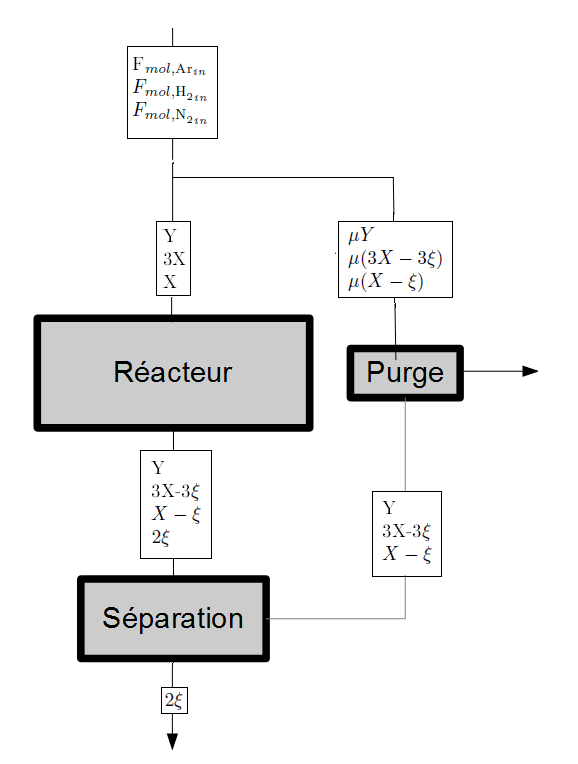
\includegraphics[scale=0.4]{Schema_synthese.png}
\caption{Aperçu des flux dans la dernière étape du procédé}
\label{Schema_synthese}
\end{figure}

Le Tableau \ref{Tableau} illustre la réaction incomplète prenant place dans le réacteur en prenant en compte le fait que les réactifs sont introduits de manière stœchiométrique. Notons  que, étant donné que le flux de \ce{NH3} produit est un paramètre, le degré d'avancement $\xi$ de notre réaction n'est déjà plus une inconnue: $2\xi = F_{mol,\ce{NH3}_{out}}$. Il apparaît que le nombre total de gaz en réaction vaut $4X-2\xi+Y$. 

\begin{table}[ht!]
\begin{center}
\begin{tabular}{|c|c|c|c|}
\hline
& \multicolumn{1}{c!{\makebox[0pt]{+}}}{\ce{N2}}
& \multicolumn{1}{c!{\makebox[0pt]{$\rightarrow$}}}{\ce{3H2}}
& \ce{2NH3} \\
\hline
$n_i$ & $X$ & $3X$ & $0$ \\
\hline
$n_f$ & $X-\xi$ & $3X - 3\xi $ & $2\xi$ \\\hline
\end{tabular}
\end{center}
\caption{Tableau d'avancement de la synthèse de l'ammoniac}
\label{Tableau}
\end{table}

En tenant compte de la réinjection, nous pouvons exprimer ce qui rentre dans le réacteur. Les équations suivantes ont été obtenues à l'aide de la Figure \ref{Schema_synthese}. Dans la suite de notre raisonnement, nous chercherons à trouver une expression des flux molaires des différents réactifs. Notons que $\mu$ est le pourcentage de purge, un paramètre que nous poserons.

\begin{empheq}[left=\empheqlbrace]{align}
& F_{mol,\ce{Ar}_{in}} + \mu Y = Y \label{eq:1}\\
& F_{mol,\ce{N2}_{in}} + \mu (X-\xi) = X \label{eq:2}\\
& F_{mol,\ce{H2}_{in}} + \mu (3X - 3\xi) = 3X\label{eq:3}
\end{empheq}

À partir du Tableau \ref{Tableau} et de quelques simplifications, nous sommes en mesure d'exprimer la constante d'équilibre $K(T)$. Dans cette expression, $p$ représente la pression dans le réacteur de synthèse. C'est bien entendu un paramètre. Nous le ferons varier dans la sous-section suivante, afin de voir son effet sur le rendement de réaction.

$$ K(T) = \left( \dfrac{4 \xi^2 \cdot (4X - 2\xi + Y)^2}{(3X-3\xi)^3 \cdot (X-\xi) \cdot p^2}\right) $$

Il ne nous reste plus qu'à exprimer $Y$ en fonction de $X$, et nous serons capables de trouver une solution pour $X$; la solution pour les différents flux molaires en découlera alors aisément. Pour ce faire, nous réutiliserons les équations présentées ci-dessus, mais également le fait que l'air est composé de 0.01\% d'\ce{Ar}, de 0.21\% d'\ce{O2} et de 0.78\% de \ce{N2}, ayant pour conséquence que $F_{mol,\ce{Ar}_{in}}= \frac{1}{78} F_{mol,\ce{N2}_{in}}$. Nous savons que:

\begin{eqnarray*}
 F_{mol,\ce{Ar}_{in}} &=& F_{mol,\ce{Ar}_{out}}  \\
   &=& (1-\mu)\cdot Y \\
\Leftrightarrow 
 Y &=& \frac{F_{mol,\ce{Ar}_{in}}}{(1-\mu)}  \\
   &=& \frac{\frac{1}{78} F_{mol,\ce{N2}_{in}}}{(1-\mu)}\\
   &=& \frac{ X - \mu (X-\xi)}{78(1-\mu)} \qquad \text{par l'équation \ref{eq:2}}
\end{eqnarray*}

Nous obtenons finalement un système de \numprint{4} équations à \numprint{4} inconnues, résoluble à l'aide de \textsc{Matlab}.
\begin{empheq}[left=\empheqlbrace]{align}
& F_{mol,\ce{Ar}_{in}}  + \mu \frac{ X - \mu (X-\xi)}{78(1-\mu)} = \frac{ X - \mu (X-\xi)}{78(1-\mu)} \\
& F_{mol,\ce{N2}_{in}} + \mu (X-\xi) = X \\
& F_{mol,\ce{H2}_{in}}  + \mu (3X - 3\xi) = 3X \\
& K(T) = \left( \dfrac{4 \xi^2 \cdot (4X - 2\xi + \frac{ X - \mu (X-\xi)}{78(1-\mu)})^2}{(3X-3\xi)^3 \cdot (X-\xi) \cdot p^2}\right) 
\end{empheq}

Une autre solution aurait été d'effectuer un boucle sur \textsc{Matlab} utilisant la récursion en réinjectant à chaque fois une partie des produits au début de la boucle. Nous avons écrit un code mettant cette technique en pratique, même si il est d'une complexité plus élevée que celui découlant des équations ci-dessus. Ce code est disponible en Annexes. Nous obtenons des résultats très similaires à ceux obtenus avec la solution analytique, mais le temps d'exécution est nettement plus long.

\subsubsection{Température et pression}

Maintenant que nous avons obtenu les équations en prenant compte la réinjection, nous sommes en mesure d'effectuer l'analyse paramétrique demandée. Cette sous-section se penche sur l'effet de la température du réacteur $T$ et la pression $p$ dans ce même réacteur. Nous ne présenterons pas ici l'effet du pourcentage de purge, étant donné que nous l'avons testé avec \textsc{Aspen+}. Voici deux graphes reprenant les résultats de notre outil de gestion \textsc{Matlab}.

\begin{figure}[ht!]
\centering
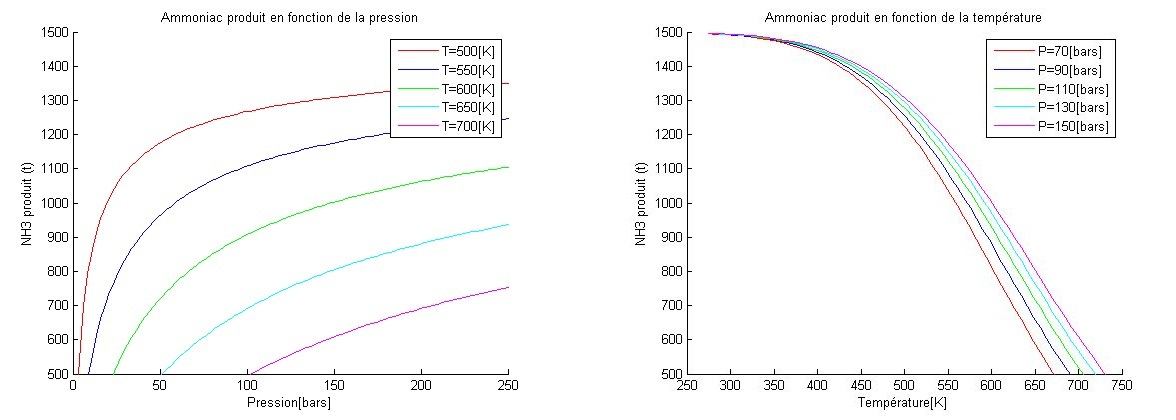
\includegraphics[scale=0.4]{fct_pression.jpg}
\caption{Quantité d'ammoniac produite en fonction de la température et de la pression.}
\label{fct_pression}
\end{figure}

Les résultats obtenus concordent avec nos prédictions: une augmentation de pression induit une augmentation de production d'ammoniac; tandis qu'une augmentation de température induit une
diminution de production.

\paragraph{} Notons que nous avons seulement considéré les contraintes thermodynamiques, sans nous préoccuper des contraintes
cinétiques. Or, ces contraintes cinétiques ont déterminé nos choix de gamme de pression et de température. Nous nous
devons donc d'y apporter quelques explications supplémentaires.

La réaction de production d'ammoniac doit se faire à l'aide d'un catalyseur. Ce catalyseur contient généralement de
l'hydroxyde de potassium \ce{KOH}, il permet d'accélérer la réaction, et il a besoin d'une température minimale de \unit{400}{\celsius}
pour être efficace. Nous avons cependant commencé l'étude paramétrique à partir de la température ambiante. Nous nous sommes
arrêtés à \unit{700}{\celsius} pour la clarté des graphes, et parce que la réaction \textsc{Haber-Bosh} se produit généralement à \unit{500}{\celsius}.
En ce qui concerne la pression, étant donné que la réaction \textsc{Haber-Bosh} se produit généralement entre \unit{100}{\bbar} et \unit{1000}{\bbar},
nous avons analysé nos résultats dans cette gamme, et nous avons conclu qu'une pression de \unit{250}{\bbar} était déjà
suffisante pour avoir un bon rendement. Augmenter d'avantage la pression n'est selon nous pas vraiment rentable économiquement parlant.


\subsubsection{Optimisation}
Nous sommes maintenant en mesure de choisir une température et une pression favorisant la réaction. De par
toute la discussion ci-dessus nous conseillerions une température de \unit{500}{\celsius}, et une pression aux environs de \unit{200}{\bbar}. Mettons encore une fois l'accent sur l'importance de la réinjection des réactifs: nonobstant ce choix de pression et de température optimal, nous ne calculons un rendement sans réinjection que de 25\%. Comparé au rendement de 98\% avec réinjection, c'est effectivement très peu.


\subsection{Analyse paramétrique avec \textsc{Aspen+}}
\textsc{Aspen+} est un logiciel qui est utilisé dans l'industrie afin de modéliser des procédés 
chimiques et d'en faire des simulations. Dans notre cas nous nous sommes juste intéressés au dernier bloc de la réaction, 
à savoir la synthèse d'ammoniac. Pour cela nous avons modélisé un flow-sheet sur \textsc{Aspen+} contenant un réacteur, un 
préchauffeur, un refroidisseur, une unité flash (pour la séparation des produits), un compresseur isentropique ainsi qu'un 
séparateur et un mixeur (Figure \ref{Aspen}).

\begin{figure}[ht!]
 \centering
 \includegraphics[scale=0.5]{Aspen.jpg}
 \caption{Flow-sheet réalisé avec \textsc{Apen+}}
 \label{Aspen}
\end{figure}

Pour réaliser cette simulation, nous nous sommes basés sur notre bilan de matière afin de déterminer les quantités de matières
rentrant dans le réacteur. Comme expliqué plus haut nous avons mis un séparateur afin de recycler nos produits dans le but 
d'augmenter un maximum le rendement. Vous trouverez dans la section ci-dessous la comparaison entre la simulation \textsc{Matlab} 
et \textsc{Aspen}.


\section*{Comparaison entre le modèle de notre outil de gestion et celui de Aspen+}
Il nous a été demandé dans le cadre de la seconde tâche d'analyser plus précisément la dernière étape du procédé, le réacteur de production d'ammoniac, considéré comme une "une boite noire" depuis le début du projet. Une analyse paramétrique a été réalisée avec notre outil de gestion ainsi qu'avec le logiciel Aspen+. Ce document présente les résultats et conclusions de cette dernière ainsi que la comparaison des modèles obtenus à l'aide des deux procédés.


\subsection*{Comparaison entre les deux modèles}
Dans les deux cas, nous remarquons que l'influence de la tempèrature et de la pression font évoluer le rendement dans un même sens: une augmentation de pression et une diminution de la température optimise ce dernier.
Dans les deux cas, une purge est obligatoire vu l'argon, dont la présence déplace l'équilibre au sein du réacteur. Sans quoi, la réaction ne saurait plus possible à partir d'un certain nombre de réinjection. Les résultats obtenus dans le cas des deux modèles coïncident, comme le montre les graphiques suivants:

\begin{figure}[ht!]
 \centering
 \includegraphics[scale=0.6]{graphe1.png}
 \caption{Rendement en fonction de la température}
 \label{scheme}
\end{figure}

\begin{figure}[ht!]
 \centering
 \includegraphics[scale=0.6]{graphe2.png}
 \caption{Rendement en fonction de la pression}
 \label{scheme}
\end{figure}

Les différences entre le résultat obtenu avec Aspen+ et notre outil de gestion peuvent provenir de plusieurs éléments comme les imprécision calculatoire de l'un ou l'autre logiciel. Du plus il peut aussi être dû au fait que la simulation réalisée avec Aspen+ prenait plus éléments en compte que notre outil de gestion, comme la pression présente dans les différents tuyaux. Ces restent pas ailleurs relativement petite dans la mesure où ce sont les même relation réactionnelles qui ont été utilisée.




